%%%%%%%%%%%%%%%%%%%%%%%%%%%%%%%%%%%%%%%%
% datoteka diploma-vzorec.tex
%
% vzorčna datoteka za pisanje diplomskega dela v formatu LaTeX
% na UL Fakulteti za računalništvo in informatiko
%
% vkup spravil Gašper Fijavž, december 2010
% 
%
%
% verzija 12. februar 2014 (besedilo teme, seznam kratic, popravki Gašper Fijavž)
% verzija 10. marec 2014 (redakcijski popravki Zoran Bosnić)
% verzija 11. marec 2014 (redakcijski popravki Gašper Fijavž)
% verzija 15. april 2014 (pdf/a 1b compliance, not really - just claiming, Damjan Cvetan, Gašper Fijavž)
% verzija 23. april 2014 (privzeto cc licenca)
% verzija 16. september 2014 (odmiki strain od roba)
% verzija 28. oktober 2014 (odstranil vpisno številko)
% verija 5. februar 2015 (Literatura v kazalu, online literatura)
% verzija 25. september 2015 (angl. naslov v izjavi o avtorstvu)
% verzija 26. februar 2016 (UL izjava o avtorstvu)
% verzija 16. april 2016 (odstranjena izjava o avtorstvu)
% verzija 5. junij 2016 (Franc Solina dodal vrstice, ki jih je označil s svojim imenom)


\documentclass[a4paper, 12pt]{book}
%\documentclass[a4paper, 12pt, draft]{book}  Nalogo preverite tudi z opcijo draft, ki vam bo pokazala, katere vrstice so predolge!



\usepackage[utf8x]{inputenc}   % omogoča uporabo slovenskih črk kodiranih v formatu UTF-8
\usepackage[slovene,english]{babel}    % naloži, med drugim, slovenske delilne vzorce
\usepackage[pdftex]{graphicx}  % omogoča vlaganje slik različnih formatov
\usepackage{fancyhdr}          % poskrbi, na primer, za glave strani
\usepackage{amssymb}           % dodatni simboli
\usepackage{amsmath}           % eqref, npr.
%\usepackage{hyperxmp}
\usepackage[hyphens]{url}  % dodal Solina
\usepackage{comment}       % dodal Solina

% \usepackage[pdftex, colorlinks=true,
%						citecolor=black, filecolor=black, 
%						linkcolor=black, urlcolor=black,
%						pagebackref=false, 
%						pdfproducer={LaTeX}, pdfcreator={LaTeX}, hidelinks]{hyperref}

\usepackage{color}       % dodal Solina
\usepackage{soul}       % dodal Solina
\usepackage[numbers]{natbib}  % dodal Solina

%%%%%%%%%%%%%%%%%%%%%%%%%%%%%%%%%%%%%%%%
%	DIPLOMA INFO
%%%%%%%%%%%%%%%%%%%%%%%%%%%%%%%%%%%%%%%%
\newcommand{\ttitle}{Uporaba diskretne kosinusne transformacije pri kompresiji signalov}
\newcommand{\ttitleEn}{Diploma thesis sample}
\newcommand{\tsubject}{\ttitle}
\newcommand{\tsubjectEn}{\ttitleEn}
\newcommand{\tauthor}{Gregor Šraj}
\newcommand{\tkeywords}{računalnik, računalnik, računalnik}
\newcommand{\tkeywordsEn}{computer, computer, computer}


%%%%%%%%%%%%%%%%%%%%%%%%%%%%%%%%%%%%%%%%
%	HYPERREF SETUP
%%%%%%%%%%%%%%%%%%%%%%%%%%%%%%%%%%%%%%%%
% \hypersetup{pdftitle={\ttitle}}
% \hypersetup{pdfsubject=\ttitleEn}
% \hypersetup{pdfauthor={\tauthor, matjaz.kralj@fri.uni-lj.si}}
% \hypersetup{pdfkeywords=\tkeywordsEn}


 


%%%%%%%%%%%%%%%%%%%%%%%%%%%%%%%%%%%%%%%%
% postavitev strani
%%%%%%%%%%%%%%%%%%%%%%%%%%%%%%%%%%%%%%%%  

\addtolength{\marginparwidth}{-20pt} % robovi za tisk
\addtolength{\oddsidemargin}{40pt}
\addtolength{\evensidemargin}{-40pt}

\renewcommand{\baselinestretch}{1.3} % ustrezen razmik med vrsticami
\setlength{\headheight}{15pt}        % potreben prostor na vrhu
\renewcommand{\chaptermark}[1]%
{\markboth{\MakeUppercase{\thechapter.\ #1}}{}} \renewcommand{\sectionmark}[1]%
{\markright{\MakeUppercase{\thesection.\ #1}}} \renewcommand{\headrulewidth}{0.5pt} \renewcommand{\footrulewidth}{0pt}
\fancyhf{}
\fancyhead[LE,RO]{\sl \thepage} 
%\fancyhead[LO]{\sl \rightmark} \fancyhead[RE]{\sl \leftmark}
\fancyhead[RE]{\sc \tauthor}              % dodal Solina
\fancyhead[LO]{\sc Diplomska naloga}     % dodal Solina


\newcommand{\BibTeX}{{\sc Bib}\TeX}

%%%%%%%%%%%%%%%%%%%%%%%%%%%%%%%%%%%%%%%%
% naslovi
%%%%%%%%%%%%%%%%%%%%%%%%%%%%%%%%%%%%%%%%  


\newcommand{\autfont}{\Large}
\newcommand{\titfont}{\LARGE\bf}
\newcommand{\clearemptydoublepage}{\newpage{\pagestyle{empty}\cleardoublepage}}
\setcounter{tocdepth}{1}	      % globina kazala

%%%%%%%%%%%%%%%%%%%%%%%%%%%%%%%%%%%%%%%%
% konstrukti
%%%%%%%%%%%%%%%%%%%%%%%%%%%%%%%%%%%%%%%%  
\newtheorem{izrek}{Izrek}[chapter]
\newtheorem{trditev}{Trditev}[izrek]
\newenvironment{dokaz}{\emph{Dokaz.}\ }{\hspace{\fill}{$\Box$}}

%%%%%%%%%%%%%%%%%%%%%%%%%%%%%%%%%%%%%%%%%%%%%%%%%%%%%%%%%%%%%%%%%%%%%%%%%%%%%%%
%% PDF-A
%%%%%%%%%%%%%%%%%%%%%%%%%%%%%%%%%%%%%%%%%%%%%%%%%%%%%%%%%%%%%%%%%%%%%%%%%%%%%%%


%%%%%%%%%%%%%%%%%%%%%%%%%%%%%%%%%%%%%%%% 
% define medatata
%%%%%%%%%%%%%%%%%%%%%%%%%%%%%%%%%%%%%%%% 
\def\Title{\ttitle}
\def\Author{\tauthor, matjaz.kralj@fri.uni-lj.si}
\def\Subject{\ttitleEn}
\def\Keywords{\tkeywordsEn}

%%%%%%%%%%%%%%%%%%%%%%%%%%%%%%%%%%%%%%%% 
% \convertDate converts D:20080419103507+02'00' to 2008-04-19T10:35:07+02:00
%%%%%%%%%%%%%%%%%%%%%%%%%%%%%%%%%%%%%%%% 
\def\convertDate{%
    \getYear
}

{\catcode`\D=12
 \gdef\getYear D:#1#2#3#4{\edef\xYear{#1#2#3#4}\getMonth}
}
\def\getMonth#1#2{\edef\xMonth{#1#2}\getDay}
\def\getDay#1#2{\edef\xDay{#1#2}\getHour}
\def\getHour#1#2{\edef\xHour{#1#2}\getMin}
\def\getMin#1#2{\edef\xMin{#1#2}\getSec}
\def\getSec#1#2{\edef\xSec{#1#2}\getTZh}
\def\getTZh +#1#2{\edef\xTZh{#1#2}\getTZm}
\def\getTZm '#1#2'{%
    \edef\xTZm{#1#2}%
    \edef\convDate{\xYear-\xMonth-\xDay T\xHour:\xMin:\xSec+\xTZh:\xTZm}%
}

% \expandafter\convertDate\pdfcreationdate 

%%%%%%%%%%%%%%%%%%%%%%%%%%%%%%%%%%%%%%%%
% get pdftex version string
%%%%%%%%%%%%%%%%%%%%%%%%%%%%%%%%%%%%%%%% 
\newcount\countA
\countA=\pdftexversion
\advance \countA by -100
\def\pdftexVersionStr{pdfTeX-1.\the\countA.\pdftexrevision}


%%%%%%%%%%%%%%%%%%%%%%%%%%%%%%%%%%%%%%%%
% XMP data
%%%%%%%%%%%%%%%%%%%%%%%%%%%%%%%%%%%%%%%%  
\usepackage{xmpincl}
% \includexmp{pdfa-1b}

%%%%%%%%%%%%%%%%%%%%%%%%%%%%%%%%%%%%%%%%
% pdfInfo
%%%%%%%%%%%%%%%%%%%%%%%%%%%%%%%%%%%%%%%%  
\pdfinfo{%
    /Title    (\ttitle)
    /Author   (\tauthor, damjan@cvetan.si)
    /Subject  (\ttitleEn)
    /Keywords (\tkeywordsEn)
    /ModDate  (\pdfcreationdate)
    /Trapped  /False
}


%%%%%%%%%%%%%%%%%%%%%%%%%%%%%%%%%%%%%%%%%%%%%%%%%%%%%%%%%%%%%%%%%%%%%%%%%%%%%%%
%%%%%%%%%%%%%%%%%%%%%%%%%%%%%%%%%%%%%%%%%%%%%%%%%%%%%%%%%%%%%%%%%%%%%%%%%%%%%%%

\begin{document}
\selectlanguage{slovene}
\frontmatter
\setcounter{page}{1} %
\renewcommand{\thepage}{}       % preprecimo težave s številkami strani v kazalu
\newcommand{\sn}[1]{"`#1"'}                    % dodal Solina (slovenski narekovaji)

%%%%%%%%%%%%%%%%%%%%%%%%%%%%%%%%%%%%%%%%
%naslovnica
 \thispagestyle{empty}%
   \begin{center}
    {\large\sc Univerza v Ljubljani\\%
%      Fakulteta za elektrotehniko\\% za študijski program Multimedija
%      Fakulteta za upravo\\% za študijski program Upravna informatika
      Fakulteta za računalništvo in informatiko\\%
      Fakulteta za matematiko in fiziko\\% za študijski program Računalništvo in matematika
     }
    \vskip 10em%
    {\autfont \tauthor\par}%
    {\titfont \ttitle \par}%
    {\vskip 3em \textsc{DIPLOMSKO DELO\\[5mm]         % dodal Solina za ostale študijske programe
%    VISOKOŠOLSKI STROKOVNI ŠTUDIJSKI PROGRAM\\ PRVE STOPNJE\\ RAČUNALNIŠTVO IN INFORMATIKA}\par}%
%     UNIVERZITETNI  ŠTUDIJSKI PROGRAM\\ PRVE STOPNJE\\ RAČUNALNIŠTVO IN INFORMATIKA}\par}%
%    INTERDISCIPLINARNI UNIVERZITETNI\\ ŠTUDIJSKI PROGRAM PRVE STOPNJE\\ MULTIMEDIJA}\par}%
%    INTERDISCIPLINARNI UNIVERZITETNI\\ ŠTUDIJSKI PROGRAM PRVE STOPNJE\\ UPRAVNA INFORMATIKA}\par}%
    INTERDISCIPLINARNI UNIVERZITETNI\\ ŠTUDIJSKI PROGRAM PRVE STOPNJE\\ RAČUNALNIŠTVO IN MATEMATIKA}\par}%
    \vfill\null%
% izberite pravi habilitacijski naziv mentorja!
    {\large \textsc{Mentor}: doc. dr. Tadej Kanduč\par}%
    {\vskip 2em \large Ljubljana, 2019 \par}%
\end{center}
% prazna stran
%\clearemptydoublepage      % dodal Solina (izjava o licencah itd. se izpiše na hrbtni strani naslovnice)

%%%%%%%%%%%%%%%%%%%%%%%%%%%%%%%%%%%%%%%%
%copyright stran
\thispagestyle{empty}
\vspace*{8cm}

\noindent
{\sc Copyright}. 
Rezultati diplomske naloge so intelektualna lastnina avtorja in matične fakultete Univerze v Ljubljani.
Za objavo in koriščenje rezultatov diplomske naloge je potrebno pisno privoljenje avtorja, fakultete ter mentorja.

\begin{center}
\mbox{}\vfill
\emph{Besedilo je oblikovano z urejevalnikom besedil \LaTeX.}
\end{center}
% prazna stran
\clearemptydoublepage

%%%%%%%%%%%%%%%%%%%%%%%%%%%%%%%%%%%%%%%%
% stran 3 med uvodnimi listi
\thispagestyle{empty}
\
\vfill

\bigskip
\noindent\textbf{Kandidat:} Gregor Šraj\\
\noindent\textbf{Naslov:} Uporaba diskretne kosinusne transformacije pri kompresiji signalov\\
% vstavite ustrezen naziv študijskega programa!
\noindent\textbf{Vrsta naloge:} npr. Diplomska naloga na univerzitetnem programu prve stopnje Računalništvo in informatika \\
% izberite pravi habilitacijski naziv mentorja!
\noindent\textbf{Mentor:} doc. dr. Tadej Kanduč\\

\bigskip
\noindent\textbf{Opis:}\\
Besedilo teme diplomskega dela študent prepiše iz študijskega informacijskega sistema, kamor ga je vnesel mentor. 
V nekaj stavkih bo opisal, kaj pričakuje od kandidatovega diplomskega dela. 
Kaj so cilji, kakšne metode naj uporabi, morda bo zapisal tudi ključno literaturo.

\bigskip
\noindent\textbf{Title:} Naslov diplome v angleščini

\bigskip
\noindent\textbf{Description:}\\
opis diplome v angleščini

\vfill



\vspace{2cm}

% prazna stran
\clearemptydoublepage

% zahvala
\thispagestyle{empty}\mbox{}\vfill\null\it%
\noindent
Na tem mestu zapišite, komu se zahvaljujete za izdelavo diplomske naloge. Pazite, da ne boste koga pozabili. Utegnil vam bo zameriti. Temu se da izogniti tako, da celotno zahvalo izpustite.
\rm\normalfont

% prazna stran
\clearemptydoublepage



%%%%%%%%%%%%%%%%%%%%%%%%%%%%%%%%%%%%%%%%
% kazalo
\pagestyle{empty}
\def\thepage{}% preprecimo tezave s stevilkami strani v kazalu
\tableofcontents{}


% prazna stran
\clearemptydoublepage

%%%%%%%%%%%%%%%%%%%%%%%%%%%%%%%%%%%%%%%%
% seznam kratic

\chapter*{Seznam uporabljenih kratic}  % spremenil Solina, da predolge vrstice ne gredo preko desnega roba

\begin{comment}
\begin{tabular}{l|l|l}
  {\bf kratica} & {\bf angleško} & {\bf slovensko} \\ \hline
  % after \\: \hline or \cline{col1-col2} \cline{col3-col4} ...
  {\bf CA} & classification accuracy & klasifikacijska točnost \\
  {\bf DBMS} & database management system & sistem za upravljanje podatkovnih baz \\
  {\bf SVM} & support vector machine & metoda podpornih vektorjev \\
  \dots & \dots & \dots \\
\end{tabular}
\end{comment}

\noindent\begin{tabular}{p{0.1\textwidth}|p{.4\textwidth}|p{.4\textwidth}}    % po potrebi razširi prvo kolono tabele na račun drugih dveh!
  {\bf kratica} & {\bf angleško}  & {\bf slovensko} \\ \hline
  {\bf DKT}      & Discrete cosine transform               & Diskretna kosinusna transformacija \\
  
%  \dots & \dots & \dots \\
\end{tabular}


% prazna stran
\clearemptydoublepage

%%%%%%%%%%%%%%%%%%%%%%%%%%%%%%%%%%%%%%%%
% povzetek
\addcontentsline{toc}{chapter}{Povzetek}
\chapter*{Povzetek}

\noindent\textbf{Naslov:} \ttitle
\bigskip

\noindent\textbf{Avtor:} \tauthor
\bigskip

%\noindent\textbf{Povzetek:} 
\noindent V vzorcu je predstavljen postopek priprave diplomskega dela z uporabo okolja \LaTeX. Vaš povzetek mora sicer vsebovati približno 100 besed, ta tukaj je odločno prekratek.
Dober povzetek vključuje: (1) kratek opis obravnavanega problema, (2) kratek opis vašega pristopa za reševanje tega problema in (3) (najbolj uspešen) rezultat ali prispevek magistrske naloge.

\bigskip

\noindent\textbf{Ključne besede:} \tkeywords.
% prazna stran
\clearemptydoublepage

%%%%%%%%%%%%%%%%%%%%%%%%%%%%%%%%%%%%%%%%
% abstract
\selectlanguage{english}
\addcontentsline{toc}{chapter}{Abstract}
\chapter*{Abstract}

\noindent\textbf{Title:} \ttitleEn
\bigskip

\noindent\textbf{Author:} \tauthor
\bigskip

%\noindent\textbf{Abstract:} 
\noindent This sample document presents an approach to typesetting your BSc thesis using \LaTeX. 
A proper abstract should contain around 100 words which makes this one way too short.
\bigskip

\noindent\textbf{Keywords:} \tkeywordsEn.
\selectlanguage{slovene}
% prazna stran
\clearemptydoublepage

%%%%%%%%%%%%%%%%%%%%%%%%%%%%%%%%%%%%%%%%
\mainmatter
\setcounter{page}{1}
\pagestyle{fancy}

\chapter{Uvod}
Za diplomsko nalogo iz te teme sem se odločil zaradi dokaj minimalne pokritosti te metode tekom študija iz računalništva in matematike. Ta metoda in njej podobne so temelj vse današnje komunikacije preko spleta, kjer je kompresija ključna za hitro pošiljanje podatkov. \par

V tem diplomskem delu se bomo ukvarjali z uporabo diskretne kosinusne transformacije(DKT) pri kompresiji signalov. Najprej bomo predstavili teoretično ozadje DKT. Podali bomo definicijo te metode na eni dimenziji in nato razširitev na dve dimenziji.\par 
Pri praktičnem delu se bomo osredotočili na slike, saj je na njih najenostavneje predstaviti kako deluje DKT v praksi in kakšne prihranke nam omogoča. Ideja te metode je, da obstaja med sosednjimi piksli korelacija. Te korelirane podatke želimo preslikati v nekoreliran prostor, kjer bomo prihranili prostor s tem, da bomo potrebovali manj podatkov za shranjevanje slike, kjer bomo izgubili minimalno vizualne natančnosti. S to preslikavo se izgubi nekaj podatkov, ti podatki so tisti, ki imajo visoko frekvenco. Na ta način bomo lahko shranili sliko z manj biti, kar bo za nas predstavljalo prihranek prostora. Pokazali bomo kako sliko preslikamo v prostor DKT in katere podatke odstranimo, da bo vizualno najmanjša razlika med originalno in skrčeno sliko. Iz teh preslikanih in skrčenih podatkov bomo pokazali kako pridemo nazaj do slike. Vizualno bomo predstavili kaj pomeni transformacija z DKT na sliki in kaj nam bodo predstavljali koeficienti v novem prostoru. \par
Predvsem bomo izpostavili JPEG kot format, ki uporablja DKT kot enega izmed glavnih gradnikov za krčenje slik. Implementirali bomo tudi enostavno verzijo uporabe DKT za kompresijo slik. Ti dve metodi bomo nato primerjali koliko sta uspešni in kaj so še dodatki, ki dalje skrčijo količino podatkov. Predstavili bomo tudi nekaj slabosti te metode in v katerih primerih ima ta metoda probleme. \par
Iz slik se to dokaj enostavno lahko razširi na posnetke, saj pri njih velja še več uporabnih lastnosti. Ne samo, da so korelirani sosednji piksli, korelirani so tudi piksli na istih lokacijah v zaporednih sličicah. Nekaj malega bomo povedali tudi o zvoku.


\chapter{Diskretna kosinusna transformacija}
\label{ch0}
\section{Enodimenzionalna DKT}
Najpogostejša definicija DKT enodimenzionalnega zaporedja dolžine N je:

\begin{equation}
C(u) = \alpha(u)  \sum_{x=0}^{N-1} f(x)cos[\frac{\pi(2x+1)u}{2N}],  
\label{eq:1}
\end{equation}

za \(u = 0,1,2,\ldots,N-1\). Podobno je inverzna transformacija definirana kot 

\begin{equation}
f(x) = \sum_{u=0}^{N-1} \alpha(u)C(u)cos[\frac{\pi(2x+1)u}{2N}],  
\label{eq:2}
\end{equation}

za \(x = 0,1,2,\ldots,N-1\). V definicijah \ref{eq:1} in \ref{eq:2} je \(\alpha(u)\) definiran kot 

\begin{equation}
\alpha(u)=
    \begin{cases}
          \sqrt{\frac{1}{N}} & \text{za $u=0$} \\
          \sqrt{\frac{2}{N}} & \text{za $u\neq 0$} \\
    \end{cases}
\label{eq:3}
\end{equation}

Iz \ref{eq:1} očitno sledi, da če je \(u = 0\) je 
\(C(u) = \sqrt{\frac{1}{N}} \sum_{x=0}^{N-1} f(x)\). Torej je prvi transformacijski koeficient povprečna vrednost vzorčnega zaporedja. V literaturi se ta vrednost običajno imenuje DC koeficient. Vsi ostali koeficienti se imenujejo AC koeficienti. \par
Za idejo kako to zgleda lahko izpustimo komponenti \(f(x)\) in \(\alpha(u)\) v \ref{eq:1}. Izris grafa  \(\sum_{x=0}^{N-1}cos[\frac{\pi(2x+1)u}{2N}]\) za \(N=8\) in različne vrednosti \(u\) je prikazan v sliki \ref{pic1}. V skladu s prejšnjimi opazkami je pri krivulji zgoraj levo (\(u=0\)) izrisana konstantna(DC) vrednost, medtem ko druge krivulje (\(u=1,2,\ldots,7\)) dajo krivulje z vedno višjimi frekvencami. Te krivulje se kličejo kosinusne bazne funkcije. Te bazne funkcije so ortogonalne. Iz tega sledi, da pri množenju katerekoli krivulje iz slike \ref{pic1} z drugo krivuljo in nato seštevanju preko vseh vzorčnih točk nam vrne ničelno(skalarno) vrednost. Množenje katerekoli krivulje iz slike \ref{pic1} same s sabo in nato seštevanju nam vrne konstantno(skalarno) vrednost. Ortogonalne krivulje so neodvisne, torej nobene od baznih funkcij ne moramo izraziti kot kombinacijo drugih baznih funkcij.

\begin{figure}[h]
\begin{center}
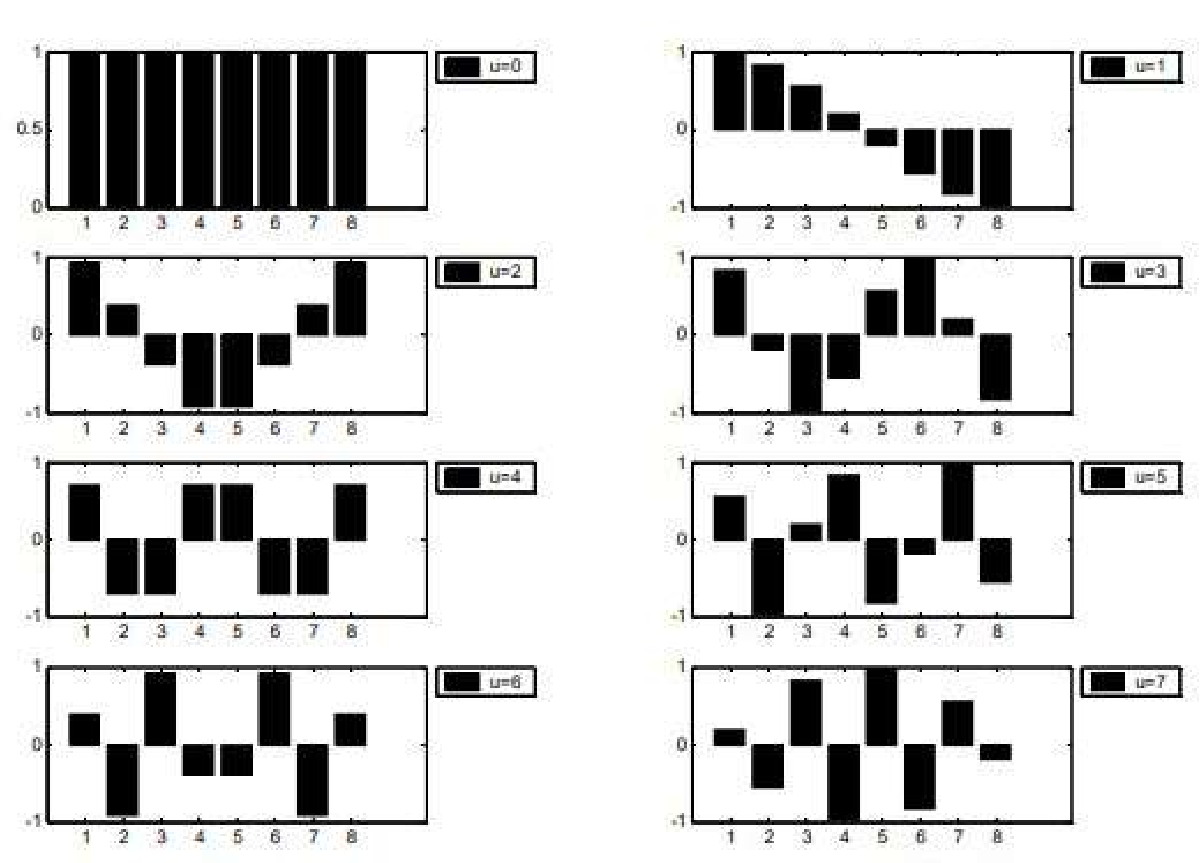
\includegraphics[width=0.6\textwidth]{slike/slika_1.pdf}
\end{center}
\caption{Enodimenzionalne kosinusne bazne funkcije (\(N=8\)).}
\label{pic1}
\end{figure}








\section{Dvodimenzionalna DKT}



%\subsection{}


\chapter{Implementacije diskretne kosinusne transformacije za slike}
\label{ch2}

\section{JPEG}

\section{Lastna implementacija}

\section{Primerjava implementacij}

\section{Slabosti diskretne kosinusne transformacije}


\chapter{Uporaba diskretne kosinusne transformacije}
\label{ch1}

\section{Slike}




\cleardoublepage
\addcontentsline{toc}{chapter}{Literatura}
\bibliography{literatura}
\bibliographystyle{plainnat}

\end{document}

